This layer is active when the user is logged in to the app and wants to add item. Once on the Add Item layer user is presented with option of entering the item description. The main task of this layer is to take product, find the suitable space for the product, generate the QR and save it in the database for future retrieval purpose.
\subsection{Item Description}
This SubSystem deals with taking the item description from user. Variety of options are provided for inputting the item. User can use the camera in the cellphone to 

\begin{figure}[h!]
	\centering
 	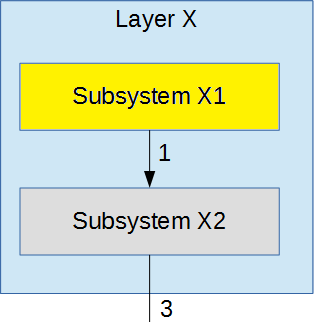
\includegraphics[width=0.60\textwidth]{images/subsystem}
 \caption{Example subsystem description diagram}
\end{figure}

\subsubsection{Assumptions}
These are the following assumptions made about this subsection:
\begin{itemize}
    \item 
\end{itemize}

\subsubsection{Responsibilities}
Each of the responsibilities/features/functions/services of the subsystem as identified in the architectural summary must be expanded to more detailed responsibilities. These responsibilities form the basis for the identification of the finer-grained responsibilities of the layer's internal subsystems. Clearly describe what each subsystem does.

\subsubsection{Subsystem Interfaces}
Each of the inputs and outputs for the subsystem are defined here. Create a table with an entry for each labelled interface that connects to this subsystem. For each entry, describe any incoming and outgoing data elements will pass through this interface.

\begin {table}[H]
\caption {Subsystem interfaces} 
\begin{center}
    \begin{tabular}{ | p{1cm} | p{6cm} | p{3cm} | p{3cm} |}
    \hline
    ID & Description & Inputs & Outputs \\ \hline
    \#xx & Description of the interface/bus & \pbox{3cm}{input 1 \\ input 2} & \pbox{3cm}{output 1}  \\ \hline
    \#xx & Description of the interface/bus & \pbox{3cm}{N/A} & \pbox{3cm}{output 1}  \\ \hline
    \end{tabular}
\end{center}
\end{table}

\subsection{Subsystem 2}
Repeat for each subsystem

\subsection{Subsystem 3}
Repeat for each subsystem

